\documentclass{article}

% if you need to pass options to natbib, use, e.g.:
%     \PassOptionsToPackage{numbers, compress}{natbib}
% before loading neurips_2019

% ready for submission
% \usepackage{neurips_2019}

% to compile a preprint version, e.g., for submission to arXiv, add add the
% [preprint] option:
    % \usepackage[preprint]{neurips_2019}

% to compile a camera-ready version, add the [final] option, e.g.:
\usepackage[final]{neurips}

% to avoid loading the natbib package, add option nonatbib:
    % \usepackage[nonatbib]{neurips_2019}
\usepackage{multicol}
\usepackage{float}
\usepackage[center]{caption}

\usepackage[utf8]{inputenc} % allow utf-8 input
\usepackage[T1]{fontenc}    % use 8-bit T1 fonts
\usepackage{hyperref}       % hyperlinks
\usepackage{url}            % simple URL typesetting
\usepackage{booktabs}       % professional-quality tables
\usepackage{amsfonts}       % blackboard math symbols
\usepackage{nicefrac}       % compact symbols for 1/2, etc.
\usepackage{microtype}      % microtypography
\usepackage{graphicx}
\usepackage{amsmath}
\usepackage{xepersian}

\settextfont{XB Yas.ttf}

\title{
پیاده‌سازی الگوریتم
\lr{Paxos}
با
\lr{TLA+}}


% The \author macro works with any number of authors. There are two commands
% used to separate the names and addresses of multiple authors: \And and \AND.
%
% Using \And between authors leaves it to LaTeX to determine where to break the
% lines. Using \AND forces a line break at that point. So, if LaTeX puts 3 of 4
% authors names on the first line, and the last on the second line, try using
% \AND instead of \And before the third author name.

\author{%
  امیرحسین مهدی‌نژاد\\
  شماره دانشجویی 810800058\\
  \texttt{mahdinejad@ut.ac.ir} \\
  % examples of more authors
  % \And
  % Coauthor \\
  % Affiliation \\
  % \texttt{email} \\
  % \AND
  % Coauthor \\
  % Affiliation \\
  % Address \\
  % \texttt{email} \\
}

% create title (includes both anonymized and non-anonymized versions)
% \providecommand{\@makepertitle}{}
% \newcommand{\makepertitle}{%
%   \vbox{%
%     \hsize\textwidth
%     \linewidth\hsize
%     \vskip 0.1in
%     \toptitlebar
%     \centering
%     {\LARGE\bf \@title\par}
%     \bottomtitlebar
%       \def\And{%
%         \end{tabular}\hfil\linebreak[0]\hfil%
%         \begin{tabular}[t]{c}\bf\rule{\z@}{24\p@}\ignorespaces%
%       }
%       \def\AND{%
%         \end{tabular}\hfil\linebreak[4]\hfil%
%         \begin{tabular}[t]{c}\bf\rule{\z@}{24\p@}\ignorespaces%
%       }
%       \begin{tabular}[t]{c}\bf\rule{\z@}{24\p@}\@author\end{tabular}%
%     \vskip 0.3in \@minus 0.1in
%   }
% }

\begin{document}


\begin{minipage}{0.1\textwidth}% adapt widths of minipages to your needs

\includegraphics[width=1.1cm]{Photos/UT_logo.png}
\end{minipage}%
\hfill%
\begin{minipage}{0.9\textwidth}\raggedleft
دانشکده فنی، دانشگاه تهران\\
سیستم‌های توزیع شده - 
دی
ماه 1400\\
\end{minipage}
% \end{}

\makepertitle

% ----------------------------------------------------------------------

% \begin{abstract}
%  این بخش از یک پاراگراف تشکیل شده است که توضیحاتی کلی در مورد مساله و راه حل شما ارائه می‌دهد.
% \end{abstract}
\begin{multicols}{2}
\section*{مقدمه}
الگوریتم
\lr{Paxos}
برای رسیدن به اجماع و
\lr{fault tolerance}
در سیستم‌های توزیع‌شده استفاده می‌شود. علت نام‌گذاری این الگوریتم در اولین مقاله‌ای که توسط لمپورت ارائه شد تحت عنوان
\lr{The Part-Time Parliament}
نشئت گرفته از سیستم پارلمانی در غرب یونان
\lr{(Paxon)}
بود که از الگوریتمی مشابه برای اجرای احکام استفاده می‌کردند و همه‌ی ساکنین بر روی آخرین قوانین اتفاق نظر داشتند.

اعضای این پارلمان به صورت پراکنده برای ضیافت‌های مختلف تالار را ترک می‌کردند، منشی نداشتند و در عوض روی تخته‌ای تمام رویدادها را ثبت می‌کردند. 

در پارلمان مذکور سه نوع قانون‌گذار وجود داشت:
\begin{itemize}
    \item Proposer پیشنهاد دهنده\\
    از پیشنهادات شهروندان حمایت کرده و در تالار مطرح می‌کردند.
    \item Acceptor پذیرنده\\
    قانون‌گذارانی بودند که رای می‌دادند.
    \item Learner یادگیرنده\\
    بعد از اینکه اجماع اتفاق می‌افتاد، یادگیرنده‌ها نتیجه‌ی توافق را اجرا می‌کردند.
\end{itemize}
برای وقوع اجماع، اکثریت
\lr{(majority)}
پذیرنده‌ها باید با لایحه‌ی جدید موافقت می‌کردند؛ که به هر جمع حداکثری از پذیرنده‌ها
\lr{Quorum}
گفته می‌شود. نکته‌ی کلیدی اینجاست که هر دو
\lr{Quorum}
موجود باید هم‌پوشانی داشته باشند.\\
\rule{\linewidth}{1pt}

\section*{نحوه‌ی رسیدن به اجماع}
پروتکلی که پارلمان
\lr{Paxon}
اجرا می‌کرد بر پایه‌ی دو فاز آماده‌سازی و موافقت بود و تا رسیدن به اجماع این اتفاقات در هر راند رخ می‌داد:
\begin{enumerate}
    \item شهروندان با پیشنهاد دهنده صحبت می‌کردند.
    \item پیشنهاد دهنده، فرمان را به پارلمان ابلاغ می‌کرد. هر فرمان شامل یک مقدار یا محتوی دستور و همچنین یک عدد بود؛ که عدد مربوط به فرمان‌ها باید اکیدا صعودی می‌بود.
    
    بعد از پیشنهاد، پذیرنده‌ها در پارلمان بحث و گفتگو کرده و اگر در هر مقطع زمانی یک
    \lr{Quorum}
    از قانون‌گذارها در تالار وجود داشت و همه رای مثبت می‌دادند، فرمان پذیرفته شده و روی تخته‌ی همه ثبت می‌شد.
    \item بعد از توافق، یادگیرنده‌ها نتیجه را گرفته و به همه‌ی شهروندان ابلاغ می‌کردند.
\end{enumerate}
بین پروتکل پارلمان
\lr{Paxos}
و دیتابیس‌های توزیع‌شده به این صورت تناظر وجود دارد:
$$\text{قانون‌گذار} \leftrightarrow \text{سرور}$$
$$\text{شهروند} \leftrightarrow \text{برنامه client}$$
$$\text{قانون فعلی} \leftrightarrow \text{state دیتابیس}$$
\rule{\linewidth}{1pt}

\section*{شرایط مسئله}
می‌دانیم ارتباطات یک به یک و
\lr{Asynchronous}
است و همچنین
\lr{Byzantine}
در کار نیست.\\
نودها
\lr{state}
خودشان را دارند که وقتی از حالت
\lr{fail}
بیرون آمدند با بقیه هماهنگ شوند.
\lr{Paxos}
با بکارگیری
\lr{2n+1}
نود،
\lr{n}
خطا را پوشش می‌دهد.

هر نود می‌تواند
هرکدام از نقش‌ها را داشته
باشد. مثلا نود اول که هر دو نقش پیشنهاد دهنده و پذیرنده را دارد، مقداری را به همراه
\lr{identifier}
پیشنهاد دهد؛ از نود دوم و سوم و حتی از خودش که پذیرنده است می‌پرسد تا تایید شود که همه آماده هستند. پذیرنده بر اساس چیزی که دریافت کرده تصمیم گرفته و قول
\lr{(promise)}
داده و آیدی کمتر را رد می‌کند.\\
باید
\lr{value}
انتخاب شده، حمایت حداکثری
\lr{Acceptor}
ها را داشته باشد تا تصویب شود.\\
\rule{\linewidth}{1pt}

\section*{پیاده‌سازی}
پروژه از سه ماژول
\lr{Paxos}
و
\lr{Phases}
و
\lr{Invariants}
تشکیل شده‌است که قبل از اشاره به هریک از آن‌ها، متغیر‌ها و مقادیر پیش‌فرض را بشناسیم:
\begin{figure}[H]
    \centering
    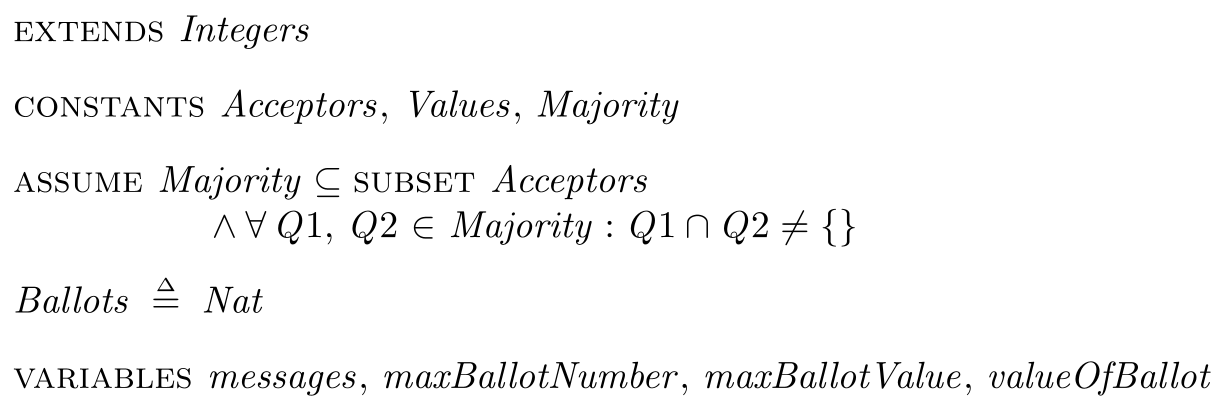
\includegraphics[width=0.99\linewidth]{Photos/HW6/vars.png}
    \caption{
    تعاریف اولیه
    }
    \label{fig:my_label}
\end{figure}
همان‌طور که پیداست در بخش
\lr{Assumption}
این تصویر، هم‌پوشانی دو
\lr{Quorum}
ذکر شده است.
\begin{itemize}
    \item \lr{messages}
    مجموعه‌ی پیام‌های ارسال‌شده
    \item \lr{maxBallotNumber}
    بیشترین عدد رای که پذیرنده در آن مشارکت داشته
    \item \lr{maxBallotValue}
    بزرگترینی که پذیرنده به آن رای داده
    \item \lr{valueOfBallot}
    مقداری که به آن رای داده شده است
\end{itemize}

\subsection*{Phases.tla}
در این ماژول فازهای الگوریتم به این شکل پیاده شدند:
\begin{figure}[H]
    \centering
    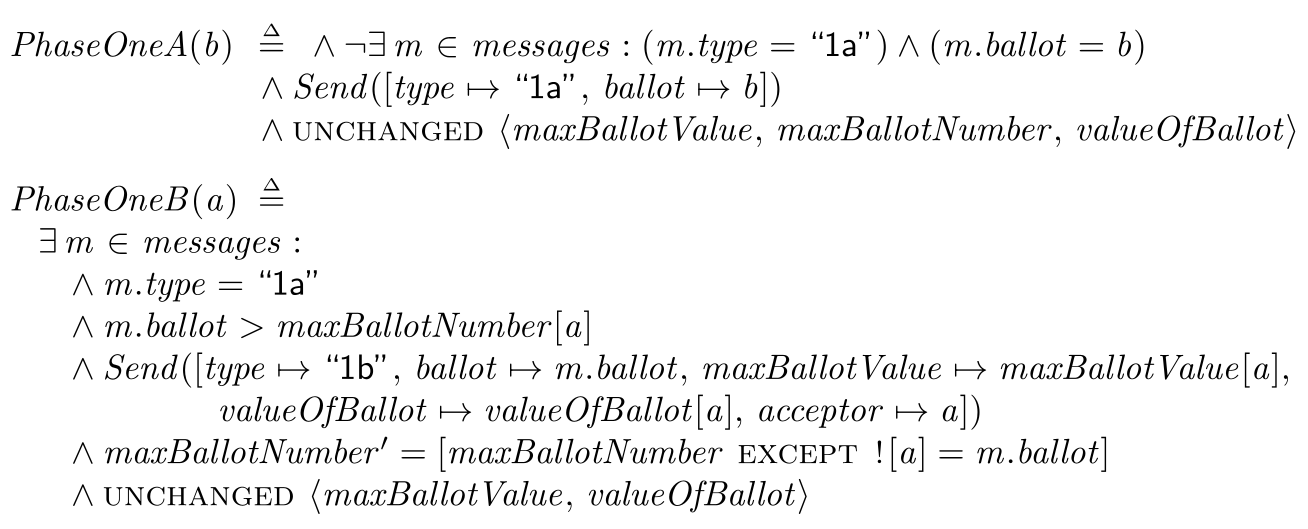
\includegraphics[width=0.99\linewidth]{Photos/HW6/one.png}
    \caption{
    فاز
    \lr{1a}
    و
    \lr{1b}
    }
    \label{fig:my_label}
\end{figure}
\begin{itemize}
    \item \lr{1a: Prepare}\\
    پیشنهاد دهنده از
    \lr{client}
    درخواست می‌گیرد و با آیدی
    \lr{N}
    آن را به جریان می‌اندازد و پیام
    \lr{prepare}
    برای همه فرستاده می‌شود.
    در صورتی این اتفاق می‌افتد که پیش‌تر برای رای
    \lr{b}
    مقدار
    \lr{"1a"}
    نیامده باشد.
    \item \lr{1b: Promise}\\
    اگر
    \lr{N}
    بزرگتر از هر آیدی از پیش دیده شده توسط پذیرنده بود، پذیرنده یک پیام
    \lr{promise}
    می‌فرستد. هر پیامی با عدد کمتر ریجکت می‌شود.\\
    در واقع همراه با
    \lr{b}
    مقدار
    \lr{"1a"}
    بزرگتر از تمام مقادیر قبل دریافت کرده است و
    \lr{promise}
    را با برچسب
    \lr{"1b"}
    می‌فرستد.
\end{itemize}
\begin{figure}[H]
    \centering
    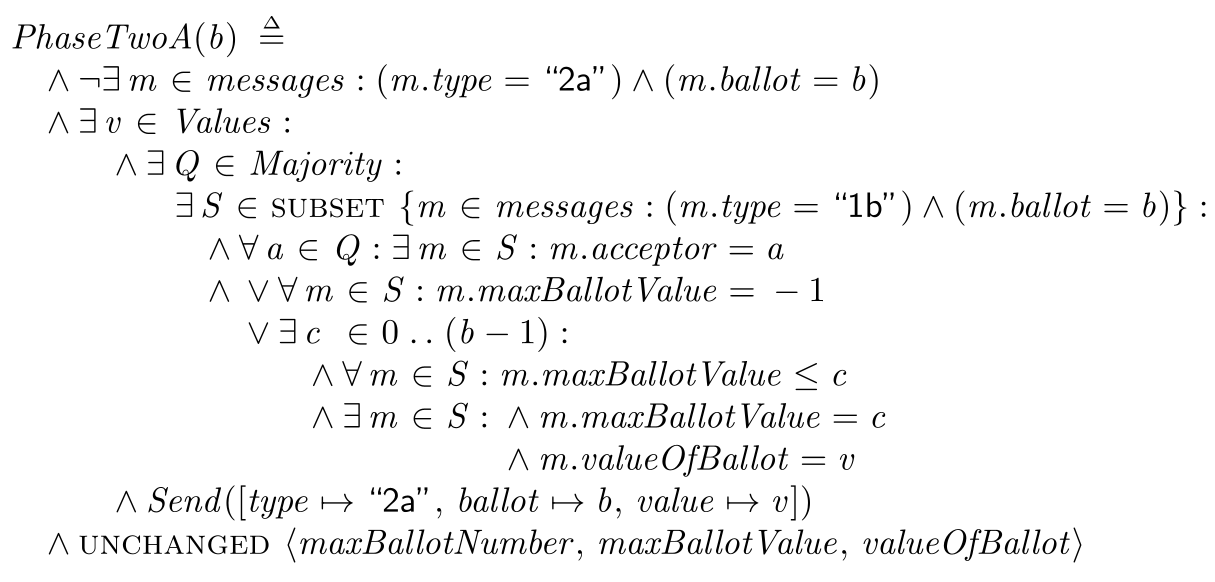
\includegraphics[width=0.99\linewidth]{Photos/HW6/twoA.png}
    \caption{
    فاز
    \lr{2a}
    }
    \label{fig:my_label}
\end{figure}
\begin{itemize}
    \item \lr{2a: Acceptance}\\
    اگر پیشنهاد دهنده از اکثریت
    \lr{promise}
    بگیرد وارد این فاز می‌شویم. مقدار تایید شده جایگزین درخواست
    \lr{client}
    می‌شود. پیشنهاد دهنده به همه‌ی پذیرنده‌ها
    \lr{Accept}
    می‌فرستد.\\
    با دریافت
    \lr{"1b"}
    از اکثریت، پیغام
    \lr{"2a"}
    به همه فرستاده می‌شود. به ازای هر رای فقط یک پیغام
    \lr{"2a"}
    خواهیم داشت.
\end{itemize}
\begin{figure}[H]
    \centering
    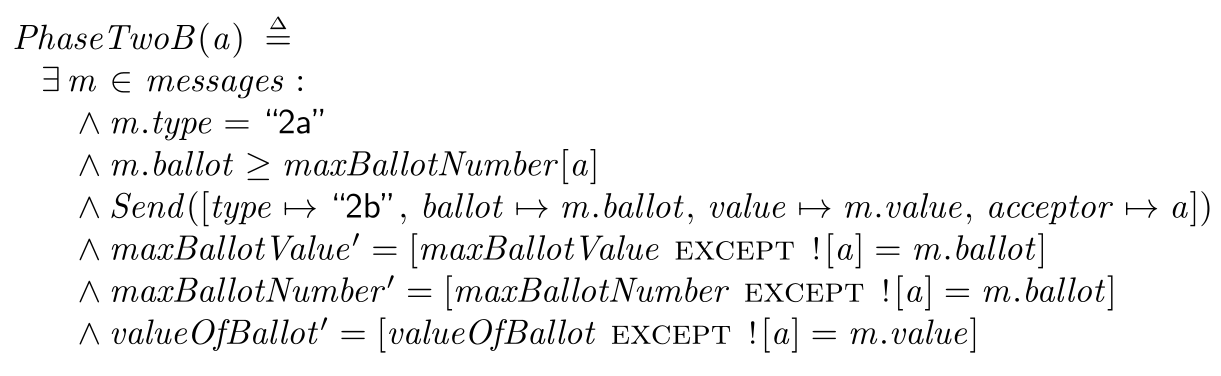
\includegraphics[width=0.99\linewidth]{Photos/HW6/twoB.png}
    \caption{
    فاز
    \lr{2b}
    }
    \label{fig:my_label}
\end{figure}
\begin{itemize}
    \item \lr{2b: Chosen}\\
    پذیرنده درخواست
    \lr{Accept}
    را می‌پذیرد اگر و تنها اگر پیام
    \lr{promise}
    برای عددی بزرگتر از
    \lr{N}
    رد نشده باشد. در صورتی که اکثریت پذیرنده‌ها درخواست را قبول کنند، مقدار انتخاب شده و قابل ویرایش مجدد نخواهد بود.
\end{itemize}
\subsection*{Invariants.tla}
در این ماژول
\lr{Invariant}
ها قرار گرفته‌اند که به بخشی از آن‌ها اشاره خواهد شد:
\begin{figure}[H]
    \centering
    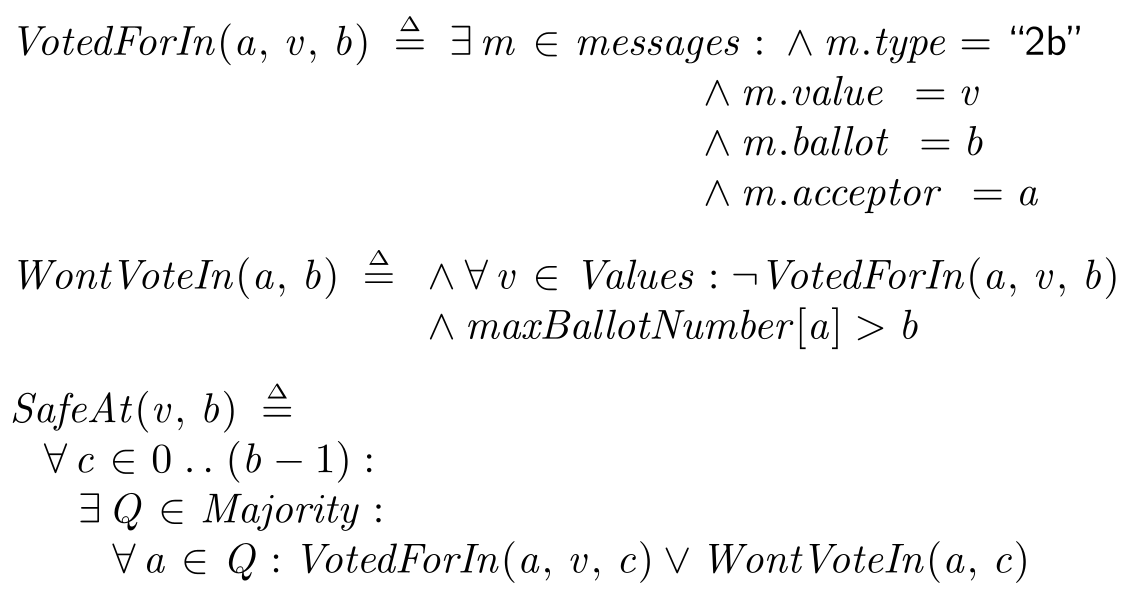
\includegraphics[width=0.99\linewidth]{Photos/HW6/voted.png}
    \caption{
    پیش‌شرط‌های رای‌دهی
    }
    \label{fig:my_label}
\end{figure}
\begin{itemize}
    \item \lr{VotedFor}\\
    یادگیرنده انتخاب شدن یک مقدار از پیام‌های نوع
    \lr{"2b"}
    را متوجه می‌شود.
    \item \lr{WontVote}\\
    پذیرنده در رای‌گیری برای یک
    \lr{ballot}
    خاص حضور نداشته است.
    \item \lr{SafeAt}\\
    هیچ مقداری مناسب‌تر از مقدار فعلی در صورتی که آیدی کمتر از
    \lr{b}
    داشته، نیست.
\end{itemize}
\subsection*{Paxos.tla}
از ماژول‌های قبلی
\lr{Instance}
ساخته شده و در این ماژول استفاده شده است:
\begin{figure}[H]
    \centering
    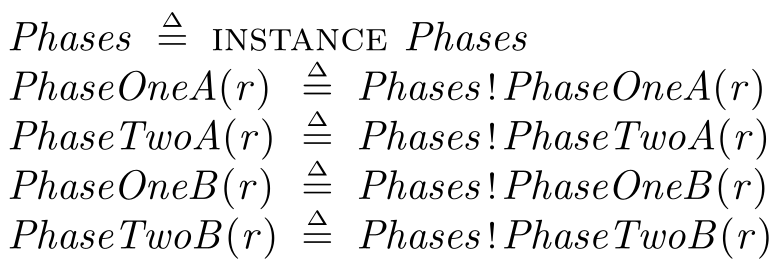
\includegraphics[width=0.60\linewidth]{Photos/HW6/instance.png}
    \caption{
    نمونه‌ی استفاده از ماژول
    \lr{Phases}
    }
    \label{fig:my_label}
\end{figure}
برای بررسی درستی برنامه از ترکیب عطفی
\lr{Invariant}
های اشاره شده در بخش‌های قبلی و همچنین شرط
\lr{consistency}
کمک می‌گیریم.
\begin{figure}[H]
    \centering
    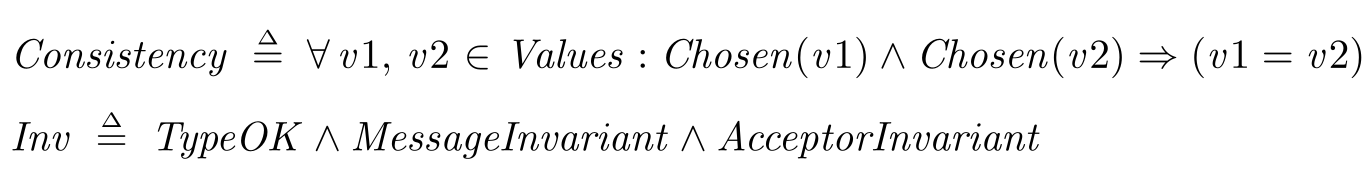
\includegraphics[width=0.99\linewidth]{Photos/HW6/inv.png}
    \caption{
    شرط سازگاری و
    \lr{Instance}
    }
    \label{fig:my_label}
\end{figure}
در اینجا
\lr{Consistency}
بدین معناست که امکان ندارد دو مقدار
\lr{v1}
و
\lr{v2}
انتخاب شده باشند یا به عبارت دیگر از این دو مقدار انتخاب شدند حتما
\lr{v1 = v2}
باشد؛ یعنی اجماع اتفاق افتاده است.\\
\rule{\linewidth}{1pt}

\section*{
بررسی اجرای برنامه
}
مجموعه‌ی ورودی‌ها یا همان
\lr{Constant}
ها بدین شکل مقداردهی شدند:
$$values \leftarrow \{"v_1", "v_2"\}$$
$$Acceptors \leftarrow \{"a1", "a2", "a3"\}$$
$$Majority \leftarrow \{\{"a_1", "a_2"\}, \{"a_1", "a_3"\}$$
$$, \{"a_2", "a_3"\}\}$$
همچنین به علت زمان‌گیر بودن اجرای برنامه، به صورت دستی
\lr{(Definition Override)}
تعریف اعداد طبیعی را تغییر داده و آن را به بازه‌ی
$[1, 3]$
محدود می‌کنیم:
$$\text{Nat} \leftarrow 1 .. 3$$
با شرایط ذکر شده برنامه کمتر از ۹۰۰هزار
\lr{state}
تولید کرده و کمتر از ۱۰ ثانیه، بدون ارور خاتمه می‌یابد.
\begin{figure}[H]
    \centering
    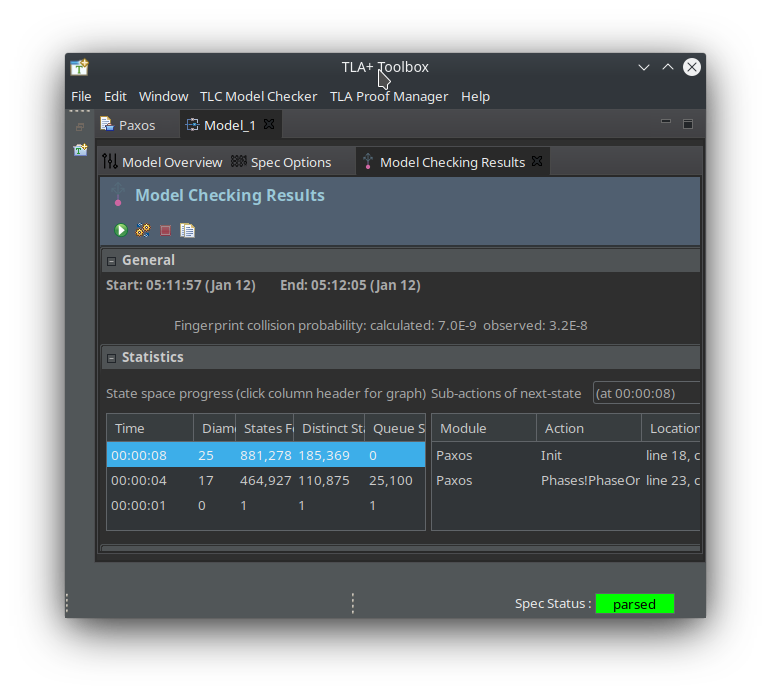
\includegraphics[width=0.99\linewidth]{Photos/HW6/toolbox.png}
    \caption{
    محیط
    \lr{toolbox}
    بعد از اجرای مدل
    }
    \label{fig:my_label}
\end{figure}
رشد مقایسه‌ها نمایی است و همین بازه اگر فقط یک واحد (تا ۴) بیشتر می‌شد، تعداد حالات مورد بررسی از ۴۰ میلیون فراتر می‌رفت.
\begin{figure}[H]
    \centering
    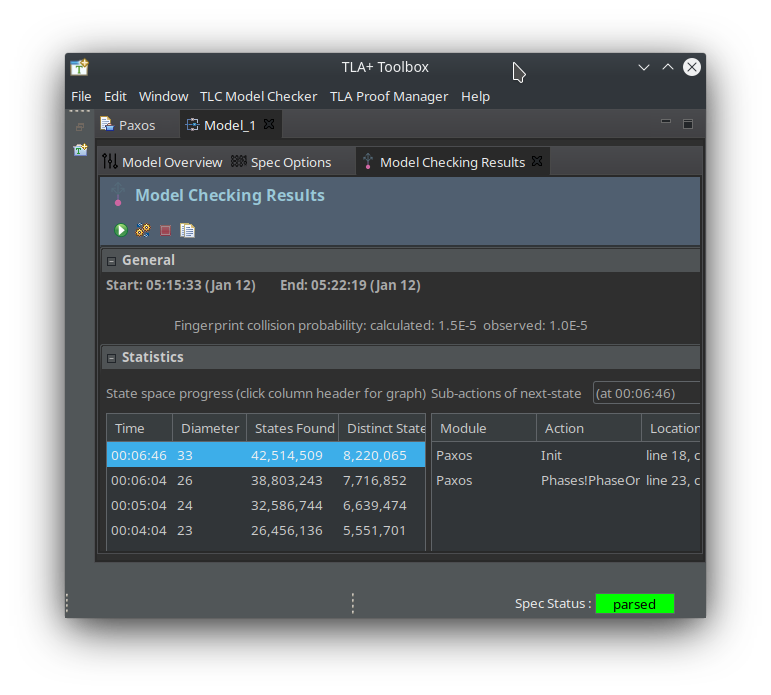
\includegraphics[width=0.99\linewidth]{Photos/HW6/four.png}
    \caption{
    اجرای مدل ضمن یک واحد بزرگتر کردن محدوده‌ی اعداد طبیعی
    }
    \label{fig:my_label}
\end{figure}
\end{multicols}
\end{document}